\chapter{Odločanje}

\section{Odločamo, ne da bi vedeli, kako to počnemo}

Odločanje običajno razumemo kot postopek izbire variante, alternative ali inačice izmed več možnih in to tako, da je izbrana varianta tista, ki najbolj ustreza našim ciljem. Poleg izbora najboljše variante včasih želimo variante tudi rangirati od najboljše do najslabše. Kadar kupujemo avto, so variante avtomobili. Pri strateškem planiranju so variante lahko različni razvojni ali investicijski scenariji. Če pa izbiramo najboljšega kandidata za neko delo, so variante ljudje. Pri odločanju se srečujemo z bogastvom človekovih vrednot, zanimanj, vedenja, sposobnosti, čustev in strasti. Zato ni čudno, če pogosto res odločamo tako, da ne vemo, kako to počnemo.

Pri sprejemanju odločitev se srečujemo z mnogimi problemi, ki izvirajo iz velikega števila dejavnikov, ki vplivajo na odločitev, iz številnih in pogosto slabo definiranih variant, iz nepopolnega poznavanje problema in ciljev, ki jih želimo uresničiti. Cilji so često tudi nasprotujoči, še posebej pri skupinskem odločanju.  Omejeni pa so tudi viri, kot je npr. čas in razpoložljivo znanje.

Z odločanjem se ukvarja vrsta znanstvenih področij in disciplin, kot so: filozofija, psihologija, ekonomija, matematika, pa tudi druge. Išče se odgovor na vprašanje, kako pomagati odločevalcu, da bi na sistematičen, organiziran in  čim lažji način prišel do kakovostne odločitve. Nastale so številne metode in tehnike za pomoč pri odločanju (Hammond et al, 2000; Krapež, Rajkovič, 2003; Bohanec, 2006; Ragsdale, 2007; Bazerman, Moore, 2009)
 
V našem pristopu bomo odločanje obravnavali na osnovi odločitvenega znanja. Zanimalo nas bo, kako človek procesira informacije in kako mu pri tem lahko pomaga sodobna informacijska in komunikacijska tehnologija. Poseben poudarek bo na ustvarjanju sinergije med človekom in informacijsko tehnologijo, kjer igrajo posebno vlogo tehnologije znanja. Človek lahko s pomočjo tehnologije odloča bolje. Poudariti pa je  treba, da končna odločitev ostaja v rokah človeka.
 
\subsection{Človek in odločanje}

Človek je tisti, ki ocenjuje, vrednoti in odloča. Ogledali si bomo nekatere dobre pa tudi slabe strani človekovega procesiranja informacij, ki lahko v veliki meri vplivajo na sprejemanje odločitev. To je pomembno predvsem zato, da bomo skušali z informacijsko tehnologijo človeku pomagati, da izkoristi svoje prednosti in zmanjša vpliv slabosti.

Čeprav je pot do odgovorov na številna vprašanja, kako delujejo naši možgani, še zelo dolga, nam obstoječa spoznanja lahko pomagajo razložiti marsikaj (Lindsay, Norman, 1977). V naš model človekovih miselnih procesov (slika~\ref{f-procesiranje-informacij}) bomo privzeli le dve vrsti človekovega spomina: kratkotrajni in dolgotrajni spomin in ju povezali s procesi potrjevanja in generiranja konceptov. Iz raziskav v psihologiji sledi, da je kapaciteta kratkotrajnega spomina le $7\pm 2$ informacijska koncepta, kot so npr. številski znaki. Če so koncepti zahtevnejši, kot je npr. kriterij cena ali varnost pri nakupu avtomobila, se kapaciteta zmanjša. Poleg relativno majhne kapacitet nas moti tudi to, da je potrebno kratkotrajni spomin nenehno osveževati, da se informacije ne izgubijo, to je, da jih ne pozabimo. 

Po drugi strani smo sposobni izjemno kakovostne obdelave informacij v kratkotrajnem spominu. Primerjamo jo lahko s hitro sočasno obravnavo, kar je izrednega pomena pri človekovem razpoznavanju vzorcev in delanju zaključkov. Sočasno razmišljamo o določeni ceni avtomobila in stopnji varnosti in ju združimo v oceno zaželenosti. Zato je kratkotrajni spomin izjemno pomemben pri ocenjevanju in odločanju. Paziti moramo, da ga naenkrat obremenimo le z nekaj informacijami. To zahteva ustrezno strukturiranje odločitvenih problemov. Osveževanje dosežemo že s svinčnikom in papirjem, medtem ko je računalniški zaslon, ki je ustrezno organiziran, še prikladnejši.

% slika 1
\begin{figure}[htbp]
\begin{center}
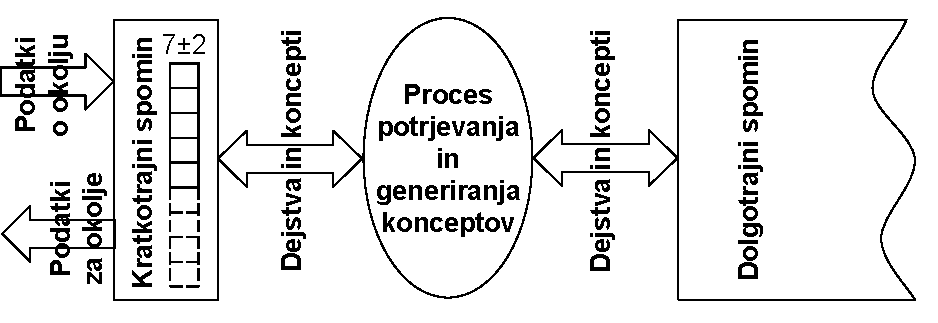
\includegraphics[width=12cm]{slike/procesiranje-informacij.pdf}
\caption{Model človekovega procesiranja informacij.}
\label{f-procesiranje-informacij}
\end{center}
\end{figure}

Dolgotrajni spomin ima za razliko od kratkotrajnega praktično neomejeno kapaciteto. Tu pa se srečujemo s problemom dostopa do informacij. Sprejet je model asociativne organiziranosti informacij. To pomeni vsebinsko povezanost konceptov. Zato moramo že na papirju ali z računalnikom podatke pripraviti tako, da so povezani v smiselne celote. Potem človek lažje izlušči pomen in ga poveže v obstoječe mreže informacij v dolgotrajnem spominu. Poseben problem dolgotrajnega spomina je preskakovanje med različnimi, ne neposredno povezanimi koncepti. Pravimo, da se pri razmišljanju ``zaplezamo'' in pozabimo na druge pomembne stvari. Spregledamo ``kraljico na šahovnici'', toda ne zato, ker bi ne znali toliko šaha, da bi lahko ugotovili, da je kraljica napadena, ampak zato, ker smo to preprosto spregledali. Seveda imamo na dlani lep pregovor: ``motiti se, je človeško''. In prav v tem pogledu si lahko z informacijsko tehnologijo bistveno pomagamo. Naredimo si opomnike v obliki spiskov ali seznamov ti. ``check lists'', za razne dejavnosti od nakupovanja do opravil v letalstvu ali zdravstvu (Gawande, 2010). V splošnem so opomniki modeli, kjer nam računalnik lahko pomembno pomaga. In tudi odločitvene model, ki vsebujejo odločitveno znanje, lahko gledamo v tej luči.

Procese, ki potekajo med obema pomnilnikoma lahko razumemo kot procese učenja pa tudi iskanja informacij. Tudi pri tem nam računalnik lahko pomaga. Posebna kategorija procesov pa je generiranje novih konceptov, kar povezujemo s pojmom ustvarjalnosti. Žal o teh procesih vemo veliko premalo. Raziskave so pokazale, da ``prazna glava'' ne more biti ustvarjalna. Potrebujemo kar nekaj let učenja, da dosežemo ta nivo. To pomeni, da ni dovolj, da je vse dosegljivo na omrežju, ampak se moramo tudi učiti in naučiti. Določiti kdaj, kako in kaj naj se na učimo, ni preprosto. Z razpoložljivo informacijsko tehnologijo so se stvari na področju vzgoje in izobraževanja bistveno spremenile. Tudi proces odločanja lahko opazujemo kot proces učenja. Zajemamo znanje, ga oblikujemo v modele, vrednotimo in razlagamo ocene. Ko se naučimo vsega, kar je potrebno v zvezi s kakim odločitvenim problemom, je naša odločitev običajno na dlani.

\subsection{Poslovni sistem in sistemi za podporo odločanju}

Kot poslovni sistem lahko smatramo podjetje, proizvodno ali storitveno, ustanovo, kot je npr. fakulteta, ali pa državo ipd. Definirajo ga vhodi in izhodi ter cilji, kot so finančna uspešnost, kakovost proizvodov oz. storitev, upoštevanje rokov in fleksibilnost, npr. v pogledu prilagajanja spremembam. Za upravljanje podjetja v smislu doseganja zastavljenih ciljev potrebujemo management, ki ga predstavlja človek oz. skupina ljudi. Management počne številne reči, vendar med vsemi opravili izstopa sprejemanje pravih odločitev. Za sprejemanje odločitev je potrebna informacija, ki jo pomaga zagotoviti informacijski sistem na osnovi podatkov o sistemu samem in okolju. Gre torej za upravljalsko zanko, ki vključuje pojme observabilnosti in kontrolabilnosti. In kje je mesto sistemov za pomoč pri odločanju? Predstavljajo most med informacijskim sistemom in upravljalci.  Podatke morajo predelati tako, da so prikladnejši za sprejemanje odločitev. (Slika~\ref{f-vloga-dss})

% slika 2
\begin{figure}[htbp]
\begin{center}
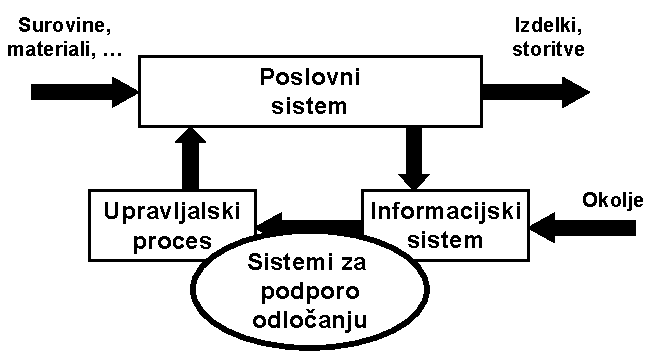
\includegraphics[width=10cm]{slike/vloga-dss.pdf}
\caption{Mesto in vloga sistemov za podporo odločanju.}
\label{f-vloga-dss}
\end{center}
\end{figure}

\subsection{Večparametrsko odločanje}

Pri odločanju nastopa množica variant $A:\; a_1, a_2\ldots a_n, \ldots$ ki je lahko tudi potencialno neskončna. Preferenčna relacija (``imam raje'') $P$ uredi množico variant $A$ po zaželenosti. Racionalna odločitev pomeni izbiro tiste variante, ki je najbolj zaželena. V splošnem je takih variant lahko več.

V odločitveni praksi običajno skušamo vpeljati funkcijo zaželenosti oz. koristnosti. Funkcija $v(a)$ izmeri stopnjo zaželenosti variante $a$, tako da za vsak par variant $a,b$ iz $A$ velja:
%
$$ a\ P\ b \Leftrightarrow v(a) > v(b) $$
%
kjer $ a\ P\ b$ pomeni, da imamo varianto $a$ rajši kot $b$. Racionalna odločitev je izbira tiste variante, ki ji funkcija $v$ izmeri največjo vrednost.

Merjenje omogoča količinsko oceno. V splošnem je merska lestvica trojica $(E, M, f)$, kjer je $E$ empirični relacijski sistem, $M$ merski relacijski sistem in $f$ osnovno merjenje, homomorfizem med $E$ in $M$.

Pri merjenju mase imamo $E=(A,T,\&)$ in $M=(\mathcal{R},>,+)$, pri čemer je dobro znano, da je masa aditivna. Pri merjenju koristnosti pa imamo v splošnem $E = (A, P)$ in $M = (D, >)$. $D$ je zaloga vrednosti, ki je lahko podmnožica realnih števil, ali pa nabor diskretnih vrednosti, npr. nezadostno, zadostno, dobro, prav dobro, odlično. Potrebno pa je poudariti, da izmerjena koristnost v splošnem ni aditivna.

Pri večparametrskem oz. večkriterijskem odločanju vpeljemo končno množico parametrov $X: x_1, \ldots, x_m$. Pri tem  $x_i: A \rightarrow D_i$, kjer je $D_i$ zaloga vrednosti $i$-tega parametra.

Varianto $a$ opišemo z naborom (vektorjem) vrednosti parametrov 

$$ a \approx x_1(a),\ x_2(a),\ \ldots,\ x_m(a) $$

Funkcijo koristnosti $v: A \rightarrow D$ nadomestimo s funkcijo $v^*$ in predpostavimo (slika~\ref{f-vecparametrsko-vrednotenje}):

$$ v(a) = v^*(x_1(a), x_2(a), \ldots , x_m(a)) $$ 

% slika 3
\begin{figure}[htbp]
\begin{center}
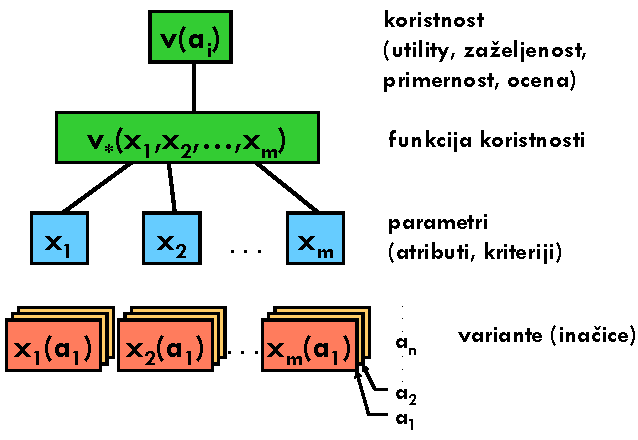
\includegraphics[width=10cm]{slike/vecparametrsko-vrednotenje.pdf}
\caption{Večparametrsko vrednotenje.}
\label{f-vecparametrsko-vrednotenje}
\end{center}
\end{figure}

\mbox{}

Pri odločanju s tveganjem se srečujemo z viri negotovosti, kot so npr. preferenčno znanje, variante in predvidevanje bodočih dogodkov. Poleg množice variant imamo tudi množico bodočih dogodkov, tj. stanj $S: s_1, s_2, \ldots s_r$. Vsak izmed bodočih dogodkov ima svojo verjetnost nastopa $p(s_j)$. Govorimo o pričakovani koristnosti, ki jo izračunamo z izrazom
%
$$u(a_i)=\sum_{j=1}^rv(a_i,s_j)*p(s_j)$$

Če verjetnosti nastopa dogodka $p(sj)$ ne moremo določiti, se soočamo s popolno negotovostjo. V tem primeru lahko uporabimo Hurwitzov kriterij	
%
$$ u(a_k) = \max_{i=1}^m (d\times \max_{j=1}^r(v(a_i,s_j) + (1-d)\times\min_{j=1}^r(v(a_i, s_j)) )$$
%
kjer za $d=0$ dobimo ti kriterij pesimističnega odločevalca za $d=1$ pa kriterij optimista. Z vmesnimi vrednostmi $d$ izrazimo našo pripravljenost za tveganje.

Pri določanju funkcije koristnosti se srečujemo s predstavitvenim problemom in problemom  enoličnosti preslikave med preferenčno relacijo in funkcijo koristnosti. Z rešitvami teh problemov se na formalnem nivoju ukvarja aksiomatski pristop k določanju funkcije koristnosti. V aksiomih zajamemo logiko odločevalca, ki zagotavlja predstavitev in enoličnost. Čeprav je ta pristop teoretično korekten, se v odločitveni praksi praviloma ne uporablja.

V praksi določamo funkcijo koristnosti enega parametra tako, da jo enostavno povemo. Predstavimo jo lahko analitično, s tabelo po točkah ali pa jo kar narišemo, kot npr. na sliki~\ref{f-koristnost-primer} za oceno primernosti starosti kandidata na merski lestvici od 0 do 100. Pomembno je, da funkcija ustreza naši preferenčni relaciji ob zastavljenih ciljih. Seveda se graf na sliki~\ref{f-koristnost-primer} močno spremeni, če gre za mladega raziskovalca, ali če ocenjujemo primernost let za predsedniškega kandidata ZDA, kjer le-ta ne sme biti mlajši od 38 let.

% slika 4
\begin{figure}[htbp]
\begin{center}
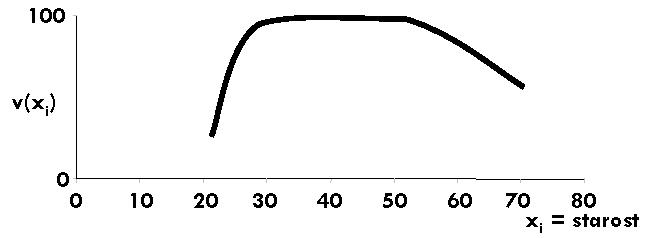
\includegraphics[width=10cm]{slike/koristnost-primer.pdf}
\caption{Funkcija koristnosti za parameter ``starost'' kandidata.}
\label{f-koristnost-primer}
\end{center}
\end{figure}
 

V praksi se pokaže, da človeku praviloma ne predstavlja problem določitev funkcije koristnosti enega parametra. Ko pa želimo izraziti koristnost dveh ali več parametrov hkrati, naletimo na težave z interpretacijo. Zato se ponavadi zatečemo k utežem, s katerimi izražamo pomembnost parametrov. Naše funkcije koristnosti so v splošnem hiperravnine. Slika~\ref{f-ocena-avta} prikazuje funkcijo koristnosti dveh parametrov, varnosti in cene, pri oceni avtomobila. Na njej je funkcija koristnosti avtomobila izračunana kot utežena vsota $\sum_{i=1}^n v(x_i) w_i$.

% slika 5
\begin{figure}[htbp]
\begin{center}
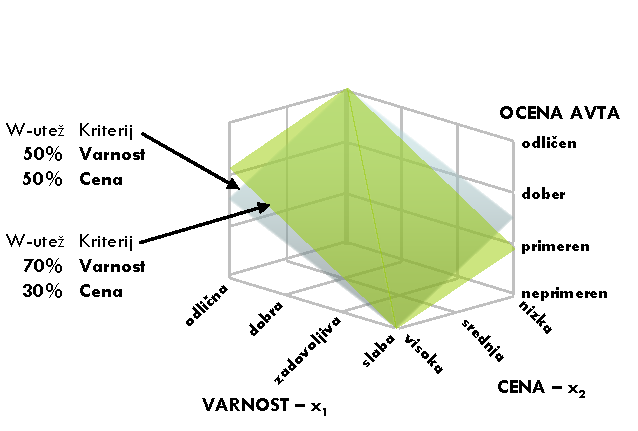
\includegraphics[width=12cm]{slike/ocena-avta.pdf}
\caption{Funkcija koristnosti dveh parametrov – ``varnost'' in ``cena''.}
\label{f-ocena-avta}
\end{center}
\end{figure}
 
Čeprav so uteži človeku nekako blizu, kot je npr. razmerje $70 : 30$ v korist varnosti (slika \ref{f-ocena-avta}), lahko linearnemu modelu očitamo, da ne sledi našim preferencam  v vseh kombinacijah vrednosti parametrov. Pri omenjenem modelu v primeru slabe varnosti in nizke cene dobimo oceno avta primeren, čeprav si avta s slabo oceno varnosti ne želimo. Rešitev bi lahko iskali v utežeh, ki bi bile spremenljive glede na vrednost parametra. Problem pa se običajno rešuje z dodatnim navajanjem omejitev nekaterih kombinacij parametrov.

V pristopu, ki je udejanjen v metodi DEX in programu DEXi, rešujemo ta problem s podajanjem funkcij koristnosti več parametrov po točkah (Efstathiou, Rajkovič, 1979; Rajkovič et al, 1988; Bohanec, Rajkovič, 1990). Izkazalo se je, da je človek sposoben konsistentno izraziti funkcijo koristnosti nekaj parametrov, običajno dveh, treh ali štirih. Pri tem pa je bistvena pomoč računalnika. Slika~\ref{f-tockovna-podaja-koristnosti} prikazuje funkcijo koristnosti parametrov cene in varnosti avtomobila, ki jo človek poda po točkah. Vsaka točka je pravilo, ki je zapisano v tabeli. Posamezno pravilo izraža preferenco z vrednostjo funkcije koristnosti v točki, ki jo določa kombinacija vrednosti parametrov kot neodvisnih spremenljivk. Človek običajno nima problemov z izražanjem in razumevanjem posameznih pravil, ki jim pravimo tudi elementarna pravila. Z računalnikom tabelo elementarnih pravil uporabimo za izračun ocene koristnosti variant. Z nadaljnjo računalniško obdelavo tabele osnovnih pravil lahko pridemo do sestavljenih (agregiranih) pravil in s tem do preglednejšega odločitvenega znanja. Z aproksimacijo funkcij koristnosti z ravnino pridemo tudi do uteži. V splošnem na osnovi tabele pravil ne omogočimo le pregledne ocene variant, ampak tudi analizo ocen.	

% slika 6
\begin{figure}[htbp]
\begin{center}
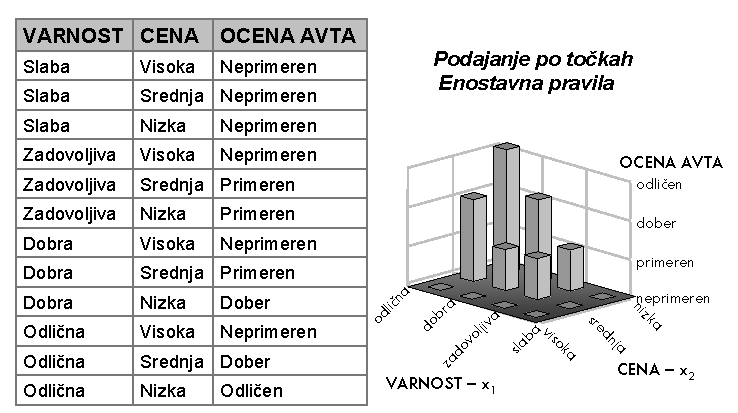
\includegraphics[width=12cm]{slike/tockovna-podaja-koristnosti.pdf}
\caption{Funkcija koristnosti podana po točkah.}
\label{f-tockovna-podaja-koristnosti}
\end{center}
\end{figure}

\section{Metode in tehnike za boljše odločanje}

Sistematično reševanje odločitvenega problema praviloma bistveno pripomore k boljši odločitvi. Pogoja za dobro odločanje sta temeljito poznavanje problema in natančno določen cilj, ki ga želimo z odločitvijo doseči. Obstojajo številne metode in tehnike, s katerimi si lahko pomagamo pri upravljanju odločitvenega znanja (Bohanec, 2006; Triantaphyllou, 2010). Gradimo odločitvene modele, ki so nam v pomoč pri vrednotenju in analizi variant. O problemu sistematično razmišljamo in si skušamo poiskati odgovor na vprašanje, zakaj je neka varianta ocenjena tako kot je in ne drugače.

Ogledali si bomo tri metode: (1) metodo ročne preglednice, (2) metodo računalniške preglednice in (3) metodo ekspertnega sistema.

Metode bomo predstavili v skladu s petimi fazami reševanja odločitvenega problema:

\begin{enumerate}
\item Identifikacija problema
\item Identifikacija kriterijev (atributov)
\begin{enumerate}
\item Seznam kriterijev
\item Struktura kriterijev (drevo kriterijev)
\item Merske lestvice
\end{enumerate}
\item Identifikacija funkcij koristnosti
\item Opis variant
\item Vrednotenje in analiza variant
\end{enumerate}

Odločitveni problem, ki ga bomo reševali, je izbira najboljšega kandidata za vodilno delovno mesto.

\subsection{Metoda ročne preglednice}

To je metoda, za katero potrebujemo le svinčnik in papir. Seznam kriterijev zapišemo tako, da najprej navedemo kriterije, ki se nam zdijo pomembnejši. Poleg vsakega parametra vpišemo tudi vrednosti, ki jih lahko zavzame in to tako, da so urejene od najslabših do najboljših, od leve proti desni. Vrednosti naj bodo naravne, tj. take, kot jih običajno uporabljamo. Npr. za znanje tujega jezika: ne, pasivno, aktivno. V računske namene lahko merske lestvice tudi poenotimo tako, da pripišemo parametrom vrednosti od 0 do 100. Tako preglednico za naš odločitveni problem izbire kandidata prikazuje slika~\ref{f-rocna-preglednica}. Tri kandidate, ki so se prijavili na razpis, opišemo z vrednostmi parametrov in jih predstavimo v preglednici.

% slika 7
\begin{figure}[htbp]
\begin{center}
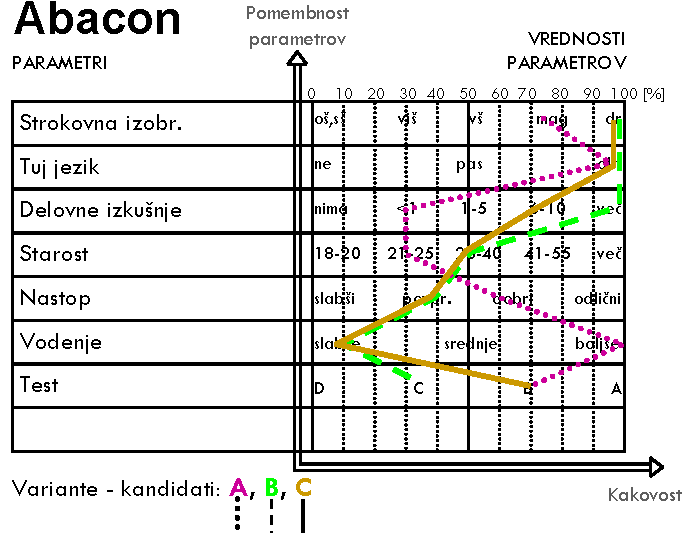
\includegraphics[width=10cm]{slike/rocna-preglednica.pdf}
\caption{Primer uporabe ročne preglednice.}
\label{f-rocna-preglednica}
\end{center}
\end{figure}

Pri tej metodi ne strukturiramo kriterijev in tudi nimamo eksplicitne funkcije koristnosti. Na nek način jo izraža pomembnost parametrov, ki pada od vrha tabele navzdol in urejenost zalog vrednosti kriterijev. Variantam tudi ne določimo končne ocene. Ta je sorazmerna s površino levo od krivulje, ki predstavlja povezavo ocen kandidata po posameznih kriterijih.

S tako predstavitvijo variant lahko sočasno primerjamo variante med seboj po posameznih kriterijih,  jih analiziramo in tolmačimo, v čem je en kandidat boljši ali slabši od drugega. S to metodo se lotevamo manjših odločitvenih problemov, kjer imamo običajno le okoli 10 kriterijev. Tudi število variant, ki jih lahko vrišemo naenkrat, je majhno. Pomembno je, da je metoda preprosta in da nudi transparenten pregled nad ocenami variant po posameznih kriterijih. 


\subsection{Metoda numerične preglednice}

Metoda predvideva uporabo računalniškega programa, npr. tipa Excel. Za naš odločitveni problem numerično preglednico prikazuje slika~\ref{f-numericna-preglednica}. V stolpcu tabele vpišemo imena kriterijev, kot smo jih identificirali že pri ročni preglednici. V stolpec poleg kriterijev vpišemo uteži pomembnosti (vplivnosti), kot smo jih prisodili vsakemu kriteriju. Merska lestvica je praviloma numerična, npr. na zaprtem intervalu od 0 do 100.

% slika 8
\begin{figure}[htbp]
\begin{center}
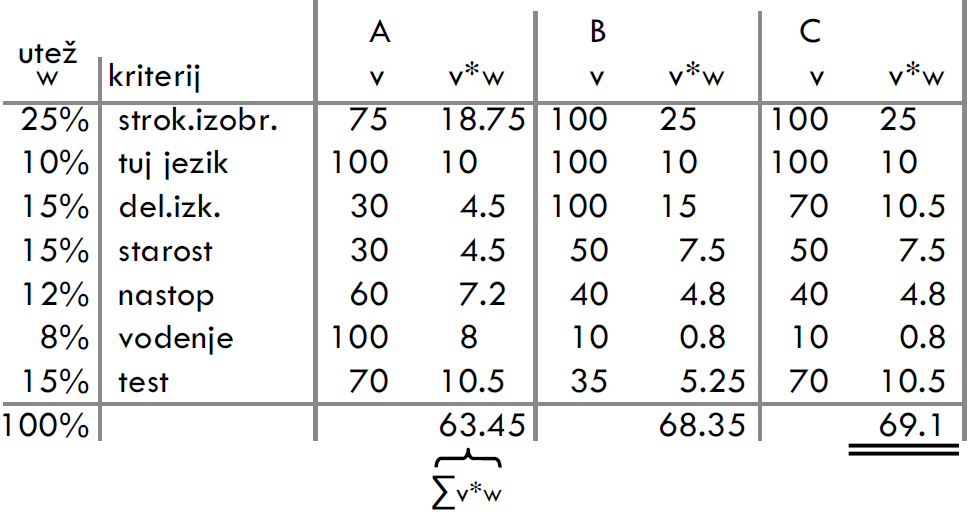
\includegraphics[width=12cm]{slike/numericna-preglednica.png}
\caption{Primer uporabe numerične preglednice.}
\label{f-numericna-preglednica}
\end{center}
\end{figure}

Če bi se odločili za strukturiranje kriterijev, bi lahko poddrevesa obravnavali v svojih tabelah. Vrednost funkcije koristnosti $v$ določimo za vsako varianto za vsak kriterij. Lahko si pomagamo s tabelo ročne preglednice na sliki~\ref{f-rocna-preglednica}, kjer smo za kriterij strokovne izobrazbe ocenili kandidata A s 75 točkami, kandidata B in C pa s 100 točkami. Končna ocena kandidata je vsota zmnožkov dodeljenih točk in uteži. Kot vidimo s slike~\ref{f-numericna-preglednica}, je po našem mnenju najboljši kandidat C, ki je dobil 69,1 točke. Glede na sprejete uteži in ocene kandidatov po posameznih kriterijih, je rezultat pravno korekten. Ni pa enostavno razložiti, v čem je dejanska razlika med kandidatoma B in C, ki številčno znaša le 0,75 točke.

Razumevanje števil in medsebojnega vpliva uteži in ocen si do določene mere lahko olajšamo s slikovnimi prikaz in ``kaj-če'' analizo. Slika~\ref{f-kaj-ce} prikazuje primer kaj-če analize, kjer so 10\% točk uteži kriterija delovne izkušnje prenesli na kriterij vodenja. Posledica te spremembe je obrnjen vrstni red kandidatov glede na numerično oceno.

% slika 9
\begin{figure}[htbp]
\begin{center}
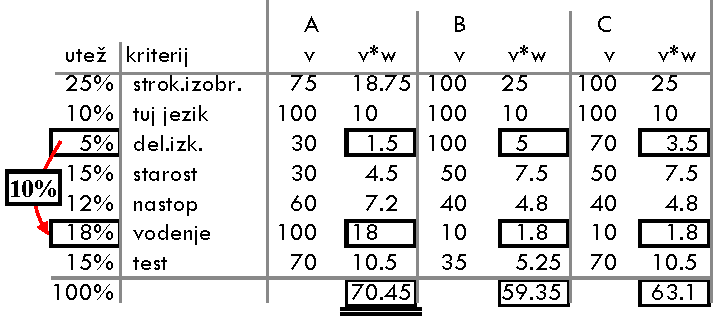
\includegraphics[width=11cm]{slike/kaj-ce.pdf}
\caption{Primer ``kaj-če'' analize.}
\label{f-kaj-ce}
\end{center}
\end{figure}

Poleg težav z interpretacijo številk, ostaja nerešen problem linearnega modela združevanja koristnosti po posameznih kriterijih v končno oceno, ki ga pooseblja utežena vsota.

Na tej osnovi so razviti številni programski pripomočki, kot je npr. HiView\footnote{\url{http://www.catalyze.co.uk/home}}, ki splošno numerično preglednico obogatijo z uporabniško prijaznimi pristopi pri obravnavi odločitvenega problema in z vizualizacijo rezultatov. Nekateri med njimi, kot npr. metoda AHP (Analytic Hierarchy Process) (Saaty, 1993), so posebej prikladni za identifikacijo uteži, s katerimi izražamo naše preference.

\subsection{Metoda ekspertnega sistema}

Metoda ekspertnega sistema skuša odločitveno znanje predstaviti kot bazo znanja ekspertnega sistema. Kot vemo, je ta v principu predstavljena podobno, kot je znanje predstavljeno na problemskem področju samem. Programsko okolje  omogoča njeno uporabo pri reševanju problema in raznovrstnih razlagah.

V ta sklop lahko uvrstimo tudi metodo DEX (Efstathiou, Rajkovič 1979; Rajkovič el al, 1988; Bohanec, Rajkovič, 1990), ki je kvalitativna večparametrska metoda. Parametri lahko zavzamejo vrednosti, ki so praviloma opisane z besedami, npr.: nesprejemljiv, sprejemljiv, dober, odličen. Numerične parametre, kot sta npr. starost ali denar, opišemo simbolično z razredi vrednosti, npr. za starost: 18-20 let, 21-25 ali npr. ceno: nizka, srednja, visoka. Pri tem definiramo razpon npr. srednje cene v ustrezni valuti. 

% slika 10
\begin{figure}[htbp]
\begin{center}
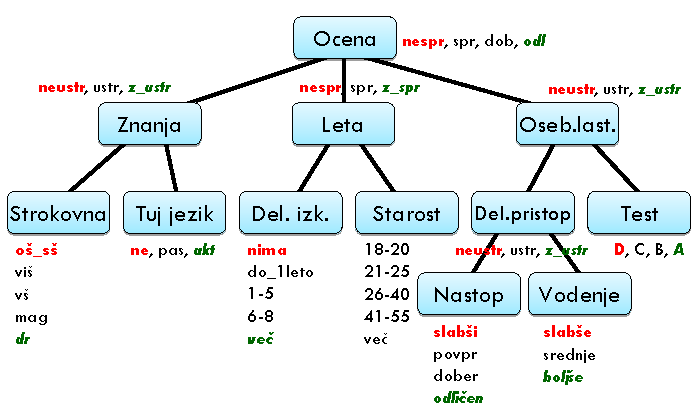
\includegraphics[width=12cm]{slike/drevo-parametrov.pdf}
\caption{Drevo parametrov z zalogami vrednosti.}
\label{f-drevo-parametrov}
\end{center}
\end{figure}
 
Slika~\ref{f-drevo-parametrov} prikazuje drevo parametrov in njihove zaloge vrednosti za naš odločitveni problem izbire najustreznejšega kandidata. Funkcije koristnosti ne definiramo s formulami oziroma utežmi, ampak po točkah s tabelami. Vsako točko lahko razumemo tudi kot preprosto pravilo tipa ``če – potem''. Na sliki~\ref{f-predstavitef-f} vidimo poleg tabele pravil za parameter delovni pristop še prostorsko predstavitev funkcije. Funkcija koristnosti je diskretna in je definirana le v prikazanih dvanajstih točkah. Funkcije so v splošnem nelinearne, pri definiranju  le-teh nam pomagajo računalniški programi kot je DEXi.

Baza odločitvenega znanja je predstavljena s kombinacijo drevesa kriterijev in pravil, s katerimi so izražene funkcije koristnosti v vozlih drevesa, ki niso listi.

% slika 11
\begin{figure}[htbp]
\begin{center}
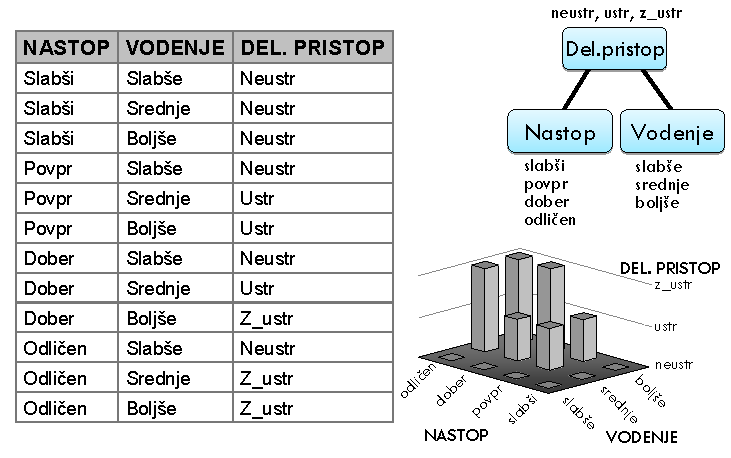
\includegraphics[width=11cm]{slike/predstavitev-f.pdf}
\caption{Predstavitev funkcije koristnosti.}
\label{f-predstavitef-f}
\end{center}
\end{figure}

Vrednotenje poteka po drevesu kriterijev od spodaj navzgor. Vsako varianto opišemo z vrednostmi kriterijev, ki so listi drevesa. Vrednosti v preostalih vozlih drevesa določajo funkcije koristnosti vse do korena drevesa, ki predstavlja končno (celostno) oceno kandidata. Slika~\ref{f-dexi} predstavlja izpis rezultatov vrednotenja  šestih kandidatov s programom DEXi. Posebej velja izpostaviti različne analize rezultatov vrednotenja in slikovne predstavitve (Jereb et al, 2003).

% slika 12
\begin{figure}[htbp]
\begin{center}
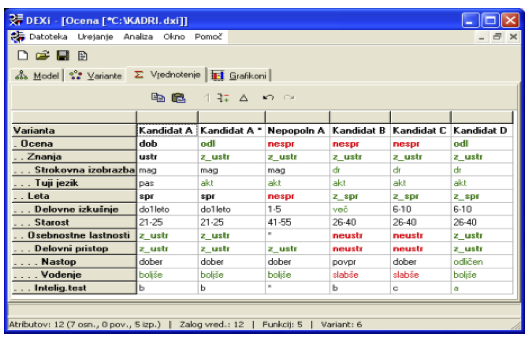
\includegraphics[width=11cm]{slike/dexi.png}
\caption{Ocena kandidatov s programom DEXi.}
\label{f-dexi}
\end{center}
\end{figure}

Metodo DEX lahko uporabimo v najzahtevnejših odločitvenih situacijah, kjer imamo opravka z velikim številom med seboj prepletenih parametrov in variant. Posebej primerna je za odločitvene situacije, kjer imamo opravka s subjektivno presojo, ki jo spremljajo parametri, ki jih je težko formalno opredeliti in natančno meriti in ocenjevati. 

Pri izražanju naših preferenc s funkcijami koristnosti imamo precej več svobode, kot jo dopuščajo linearne funkcije. Nismo omejeni le na izražanje z utežmi. Res pa je, da je prostor izražanja diskreten in relativno majhen, saj je omejen z zalogami vrednosti parametrov. Posledica tega je manjša občutljivost modela. Več variant se lahko znajde v istem ocenitvenem razredu. Če nam to ne ustreza, se lahko lotimo dodatnih analiz, kot npr. s programom Vredana\footnote{\url{http://lopes1.fov.uni-mb.si/dex/vredana/}}.
 

\section{Skupinsko odločanje in usklajevanje različnih interesov}

Odločanje v skupini predpostavlja sodelovanje oz. udeležbo (participacijo) različnih ljudi. Je proces, v katerem dva ali več subjektov vpliva drug na drugega v izvedbi odločanja. Pri tem običajno gre za odločitve, ki bodo v prihodnje zadevale sodelujoče v skupini, oz. tiste, ki jih zastopajo. Participacija vsebuje tudi idejo o različnih interesih, ki jih moramo preliti v skupno odločitev (Zarate et al, 2008).


\subsection{Zakaj skupinsko odločanje?}

Glavni smoter sodelovanja vseh, ki jih odločitev zadeva, v odločitvenem procesu, je pravica ljudi, da smejo odločati o svoji usodi. Za dosego cilja ``splošno dobrega'' prispeva širše okolje. Cilj odločitve, ki smo jo sprejeli v diskusiji, kritiki in s kompromisom, je v največji možni meri upoštevanje interesov vseh in ne le kake podskupine ali posameznika.

Pomemben razlog za skupinsko odločanje je kompleksnost odločitvenih situacij. Število elementov in zamotanost povezav med njimi je pri odločanju lahko zelo velika. Zato so v težavah tudi najboljši strokovnjaki. S sodelovanjem prizadetih ((vseh) deležnikov) se veča verjetnost, da uporabniki in ``elita'' dobijo sistem, ki ga želijo, saj gre za prispevek v fazi snovanja sistema.

Sodelovanje v skupini lahko vidimo tudi v luči managementa sprememb. Če smo pasivni spremljevalci sprememb, se jih bojimo in pogosto se jim tudi upiramo. Tisti, ki sodeluje, se nauči, kako jim biti kos. Prilagodimo sebe spremembam in spremembe sebi v skladu z dejanskimi spremembami in možnostmi.

Participacija ima tudi učno-vzgojni učinek. Če hočemo sprejeti odločitev, ki jo razumemo, razumeti pa jo moramo, če hočemo vedeti, ali je za nas dobra ali ne, moramo imeti ustrezno znanje. S sodelovanjem v skupini smo na nek način prisiljeni dokopati se do tega znanja. Ostali udeleženci nam pri tem lahko pomagajo. S sodelovanjem v skupini sprejemamo nase odgovornost odločitve. Razvija se nam čut za odgovornost, sodelovanje in sporazumevanje ter potreba po zadostnem in jasno predstavljenem znanju.


\subsection{Problemi skupinskega odločanja}

Prav je, da se vprašamo, kakšna je dejanska korist skupinskega odločanja. Če pogledamo na vloženi čas in delo, je jasno, da je sam postopek odločanja dražji. Vloženi trud in denar se obrestujeta s tem, da sprejeto odločitev tisti, ki jih zadeva, bolje razumejo in sprejemajo. To so lahko stvari, ki jih le težko kupimo z denarjem.

Nasprotniki participativnega pristopa pogosto očitajo, da z vpletanjem ``neukih'', čeprav jih odločitev zadeva, v odločanje, porazdelimo odgovornost zato, da bi zaščitili res odgovorne, ali pa da je sodelovanje ljudi le prefinjena metoda manipulacije. Morda je v teh očitkih včasih tudi nekaj resnice. Odgovor na te očitke sloni na razumljivem odločitvenem znanju. Praviloma imamo s sodelovanjem ne le možnost dostopa do tega zanja in razumevanja le-tega, ampak tudi možnost njegovega dograjevanja. Če odločamo na osnovi znanja, ki ga tudi razumemo, potem vemo zakaj odločamo tako, kot odločamo, in nas ne moti sprejemanje odgovornosti za odločitev. Tudi strah pred manipulacijo izgubi svojo osnovo.

Še nekaj besed o ustrezni organizaciji in vodenju odločitvene skupine. Osnovno vprašanje je, kako naj odločevalec sodeluje v skupini, da bodo doseženi omenjeni cilji participacije. Predpogoj je splošna ``klima'', ki mora dati vsem članom skupine občutek enakih med enakimi s skupnim ciljem rešitve odločitvenega problema. Govorimo o treh pogojih uspešne participacije: (1) motivacija, (2) nivo znanja in (3) brez sovraštva. 

Član skupine, ki ni motiviran, praviloma ne prispeva tistega, kar bi lahko. Motivacija je nemalokrat osnovana tudi  na strahu, da bi brez nas odločali v našo škodo. Nivo splošnega znanja mora biti dovolj visok, da razumemo odločitveni problem in način njegovega reševanja. Med člani odločitvene skupine ne sme biti sovražnega rivalstva.

Organizacija dela v skupini je breme, ki ga nosi predvsem vodja skupine. Ta je običajno tudi odločitveni analitik, ekspert na področju odločanja. Pomembna so znanja psihologije in sociologije ter seveda znanja s področja modeliranja in upravljanja z odločitvenimi znanji.

\subsection{Kako usklajevati različne interese?}

Povsem naravno je, da se ljudje o istih stvareh odločamo različno. Imamo različno preferenčno znanje, ki izhaja iz različne povezanosti z odločitveno situacijo, različnih vrednot in načel in iz različnega poznavanja okoliščin, pa tudi iz razlik v znanju in neznanju (nevédenju). Razmislimo o družinskem nakupu avtomobila in o razlikah v preferencah med starši in otroci.

Na osnovi preferenčnega znanja vzpostavimo preferenčno relacijo med variantami tako, da jih razporedimo po stopnji zaželenosti. Lahko pa tudi uporabimo kak model vrednotenja, da izrazimo oz. izmerimo stopnjo zaželenosti  posamezne variante npr. s točkovanjem na skali od 1 do 10. Otroci in starši ocenijo različne avtomobile različno. 

Kako iz različnih ocen variant priti do skupne odločitve? Najprej preverimo, če različne ocene ne izvirajo iz neznanja oz. nezadostnega poznavanja ciljev, variant in možnosti. Pri tem pomaga utemeljevanje svojih (različnih) preferenc. Za tem se soočimo z različnimi interesi.

Ločimo dva osnovna pristopa, ki temeljita na razliki, ki je v tem ali skupine z različnim interesi želijo ali ne želijo sodelovati med seboj pri iskanju skupne kolikor toliko smiselne in pravične odločitve oz. izbire.

Pri skupinah, ki se ne želijo posvetovati in sodelovati med seboj, lahko uporabimo kako od formalnih metod, npr. glasovanje. Vsaka izmed teh metod ima svoje prednosti in slabosti. Nobelovec Arrow (prejel Nobelovo nagrado leta 1972) je s svojim izrekom o nemogočem (Arrow et al, 2002) pokazal in dokazal, da idealne metode ni in je ne more biti. Vendar to ne negira skupinskega odločanja, ampak nas vzpodbuja k iskanju metode, ki je v dani situaciji za skupino, ki išče skupno odločitev, najprimernejša.

Če se odločimo, da vsaka interesna skupina vsaki varianti določi svojo stopnjo zaželenosti in so skupine pripravljene poiskati kompromisno rešitev, lahko uporabimo nekaj zanimivih pristopov (Lu et al, 2007). Vzemimo že omenjeni dve interesni skupini tj. (1) starše in (2) otroke pri nakupu družinskega avtomobila. Vsaka skupina oceni avtomobile, ki pridejo v poštev, glede na njihove preference na lestvici od 0 do 10. Posamezna varianta, tj. avto, je lahko predstavljena s točko s koordinatami npr. $v_1$ in $v_2$ (slika~\ref{f-primerjava-alternative}), kjer $v_1$ pomeni oceno s strani staršev, $v_2$ pa oceno s strani otrok.

% slika 13
\begin{figure}[htbp]
\begin{center}
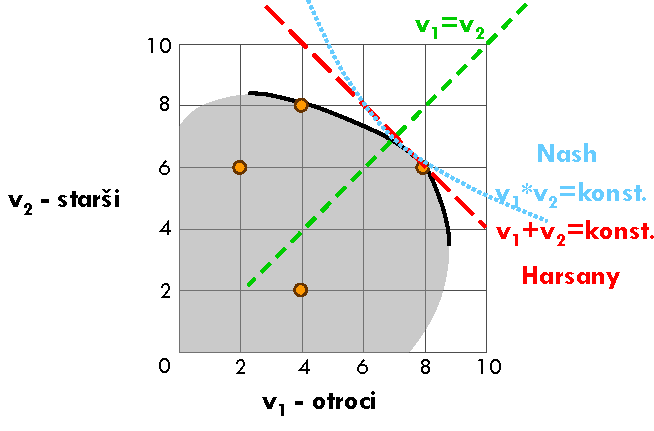
\includegraphics[width=10cm]{slike/primerjava-alternative.pdf}
\caption{Primerjava alternativ, ki jih ocenjujeta skupini z različnimi interesi.}
\label{f-primerjava-alternative}
\end{center}
\end{figure}

Smiselno je obravnavati le ne manj vredne variante, ki ležijo na debelo izvlečeni črti slike~\ref{f-primerjava-alternative}. Vse variante pod to črto so take, da lahko najdemo boljšo, tj. tako, ki ima večjo oceno ene skupine in pri tem ne manjšo druge. S tem si lahko prihranimo precej kasnejšega dela.

Odprto vprašanje ostaja, katero varianto izmed ne manj vrednih izberemo kot skupno odločitev. Če se odločimo za pristop ``enakega zadovoljstva'' to pomeni presečišče premice $v_1=v_2$. Realno bi v našem primeru iskali avto, ki bi ga otroci in starši podobno ocenili. Harsany (1955) je predlagal izbiro variante, ki maksimizira vsoto posameznih koristnosti. Njegovemu pristopu očitajo, da lahko pride do situacij, kjer se nekatere skupine dobesedno žrtvujejo v skupno dobro. Nobelovec Nash (nagrado je prejel leta 1994) je predlagal usklajevanje interesov z maksimizacijo produkta koristnosti (Nash, 1950). Z drugimi besedami, mislimo nase pa tudi na ostale. Za dobro skupno odločitev ne pride v poštev žrtveno jagnje. 

Primeri usklajevanja na sliki~\ref{f-primerjava-alternative} predstavljajo usklajevanje interesov na osnovi končnih ocen. Odločitveno znanje je izraženo le s končno oceno. Manjka nam razumevanje v pogledu izvora različnih ocen. Končna ocena je le posledica.

Za usklajevanje interesov pri izvoru različnih ocen in ne le pri posledici, tj. končni oceni, so nam lahko v posebno pomoč hierarhični večparametrski modeli (Lu et al, 2007; Triantaphyllou, 2010). Le ti imajo strukturo, imajo notranje (izpeljane) parametre in so odprti. To pomeni, da pri vrednotenju ne dajejo samo končnih ocen, pač pa je možno ``pogledati vanje'' in si ogledati, kako in zakaj je prišlo do ocen. Pogovarjamo se o posameznih parametrih, njihovih vrednostih in medsebojnih odvisnostih. Na razpolago so nam vsi elementi vrednotenja.

Iz naših izkušenj lahko povemo, da je smiselna enotna struktura modela, kljub različnim preferencam, ki izhajajo iz različnih interesov. Vsaka interesna skupina pa lahko znotraj te strukture definira svoje lastne funkcije koristnosti. Z modelom ovrednotimo variante za vsako skupino posebej. Praviloma dobimo različne ocene istih variant. Z različnostjo se ne soočimo le pri končnih ocenah, ampak opazujemo tudi vrednosti variant po posameznih notranjih parametrih. Namesto, da bi usklajevali le na nivoju končne ocene, pogledamo, kje nastopajo razlike in kakšne so. Z razlago razlik spoznamo bistvene točke razhajanja in na tej osnovi usklajujemo interese med skupinami.


\subsection{Zaključek}

Skupinsko odločanje je praviloma zahtevnejše. Rezultat tega je odločitev, ki jo ljudje lažje razumemo in jo znamo tudi bolje utemeljiti. Utemeljitev, zakaj smo se odločili tako, kot smo se in ne drugače, tudi poveča verjetnost dobre odločitve ali pa vsaj zmanjša možnost za slabo odločitev.

Razumljiva in utemeljena odločitev je tudi bistvena za smiselno uskladitev različnih interesov. Končna ocena variante je posledica številnih dejavnikov, ki so nastopili v procesu vrednotenja. Naši procesi odločanja morejo in morajo biti transparentni vse od posameznih merljivih kriterijev preko njihove agregacije do končne ocene variante.

Pri tem so nam na razpolago številni preizkušeni pristopi, metode in tehnike, ki so običajno podprte s sodobno informacijsko tehnologijo. Uporabimo jih. Razvijmo odprte in pregledne modele, da bo odločitveno znanje dostopno vsem deležnikom. Ko izbiramo najustreznejšo varianto, mislimo nase in na druge, ki jih ta odločitev zadeva.

\subsection*{Literatura}
\begin{description}
\item Arrow K. J., Sen A. K., Suzumura K., Handbook of social choice and welfare, North Holland, Amsterdam, 2002
\item Bazerman M.H., Moore D., Judgement in managerial decision making, Wiley, 2009
\item Bohanec M., Odločanje in modeli, DMFA, 2006
\item Bohanec M., Rajkovič V., DEX: an expert system shell for decision support, Sistemica 1(1), 1990: 145-157 http://wwwai.ijs.si/MarkoBohanec/pub/, Sistemica90.pdf
\item Bohanec M., Urh B., Rajkovič, V., Evaluating options by combined qualitative and quantitative methods, Acta Psychologica 80, 1992: 67-89
\item Efstathiou J., Rajkovič V., Multi-attribute decision making using a fuzzy heuristic approach, IEEE Transaction on Systems, Man and Cybernetics 9(6), 1979: 326-333
\item Gawande A., The checklist manifesto: How to get things right, Metropolitan Books, New York, 2010
\item Hammond J.S., Keeney R.L., Raiffa H., Pametne odločitve: praktični vodnik za sprejemanje boljših odločitev, Gospodarski Vestnik, Ljubljana, 2000
\item Harsanyi J., Cardinal welfare, individualistic ethics and interpersonal comparison of utility, Journal of Political Economy 63(4), 1955: 309-321
\item Jereb E., Bohanec M., Rajkovič V., DEXi - Računalniški program za večparametrsko odločanje, Uporabniški priročnik, Moderna organizacija, Kranj, 2003
\item Krapež A., Rajkovič V., Tehnologije znanja pri predmetu informatika, Zavod RS za šolstvo, Ljubljana, 2003
\item Lindsay H. P., Norman A. D., An introduction to psychology, Academic Press, New York, 1977
\item Lu J., Zhang G., Ruan D., Multi-objective decision making: Methods, software and applications with fuzzy set techniques, Imperial College Press, London, 2007
\item Nash J., Equilibrium points in n-persons games, Proceedings of the National Academy of Sciences, 36(1), 1950: 48-49
\item Ragsdale C.T., Managerial decision modelling, Thomson Higher Education, 2007
\item Rajkovič V., Bohanec M., Batagelj V., Knowledge engineering techniques for utility identification, Acta Psychologica 68(1-3), 1988: 271-286
\item Saaty T. L., Multicriteria Decision Making: The Analytic Hierarchy Process, RWS Publications, 1993
\item Triantaphyllou E., Multi-Criteria Decision Making Methods: A Comparative Study (Applied Optimization), Kluwer Academic Publishers, 2010
\item Zarate P., Belaud J. P., Camilleri G., Ravat  F. (eds.), Collaborative decision making: Perspectives and challenges, IOS Press, Amsterdam, 2008
\end{description}
